\section{Tutorial - Pi Setup and Linux Basics}
\subsection{Overview}
This practical sets out to familiarise you with the Pi and to complete a simple programming task. If you have not yet done so, setup your Pi. 

There is tons of Raspberry Pi information on the EE Wiki, with an overview page accessible \href{http://wiki.ee.uct.ac.za/RaspberryPi:Overview}{here}. It's suggested you take a look at what information is available to you.

\textbf{Due date:} See Vula

\subsection{Pre-Prac Tasks}
\begin{itemize}
\itemsep0em 
    \item Set up your Pi and ensure it's configured correctly! See the Wiki for details \href{http://wiki.ee.uct.ac.za/RaspberryPi:Installation}{http://wiki.ee.uct.ac.za/RaspberryPi:Installation}\\
    There is also a video \href{https://www.youtube.com/watch?v=2vqEQVoK58M}{here}. While it was created on Windows, the steps for setting them up are universal.\\
    \item Add internet access to your Pi. The easiest way is through WiFi, which you can read about \href{http://wiki.ee.uct.ac.za/RaspberryPi:Networking#Simple_Wifi_Connections}{here}. If you do not have access to WiFi, you can read about Ethernet passthrough \href{http://wiki.ee.uct.ac.za/RaspberryPi:Networking#Internet_Access_over_USB}{here}.
    \item Read the sections ``Inputs" and ``Outputs" on the RPi.GPIO documentation, available \href{https://sourceforge.net/p/raspberry-gpio-python/wiki/Examples/}{here.}
    %Change README - references Prac 2 
    \item Get a basic understanding of git. For details regarding git and it's usage, read through \href{http://wiki.ee.uct.ac.za/Git}{http://wiki.ee.uct.ac.za/Git}
    \item Clone the prac source files into your own directory from \href{https://github.com/UCT-EE-OCW/EEE3096S-Pracs-2020}{https://github.com/UCT-EE-OCW/EEE3096S-Pracs-2020}. The prac we're concerned with is Prac 3! There's a walkthough on this later on if you're uncertain.

\end{itemize}

\subsection{Pre-prac Requirements}
This section covers what you will need to know before starting the practical.
\begin{itemize}
    \item Have your Raspberry Pi Set up correctly.
    \item Have an understanding of how you can edit text files on the Pi using an editor such as vim or nano.
    \item Have a basic understanding of Git.
\end{itemize}

\subsection{Hardware Required}
\begin{table}[H]
\begin{tabular}{ll}
\begin{tabular}[c]{@{}l@{}}\tabitem Raspberry Pi with configured SD Card\\ \tabitem A breadboard\\ \tabitem 1 x push button\\ \end{tabular} & \begin{tabular}[c]{@{}l@{}} \tabitem 1 x LED\\ \tabitem 1 x Resistor\\ \tabitem Dupont Wires\\\end{tabular} \\
\end{tabular}%
\end{table}

\subsection{Outcomes of this Practical}
You will learn about the following topics:
\begin{table}[H]
\begin{tabular}[c]{@{}l@{}}\tabitem Basic GPIO Usage\\ \tabitem Interrupts\\ \tabitem Debouncing \end{tabular}
\begin{tabular}[c]{@{}l@{}}\tabitem Git\\ \tabitem Bash\\ \tabitem SSH\\ \end{tabular}  
\end{table}

\subsection{Deliverables}
At the end of this tutorial, you must:
\begin{itemize}
    \item Submit a single PDF with your screenshots and answers to the questions from the Terminal task to Vula. Ensure the PDF contains a link to your GitHub repo for the Programming task. 
\end{itemize}

\subsection{Walkthrough}
This tutorial consists of two parts - a terminal task and a programming task. 

\subsubsection{Terminal Task}
\label{sec:Prac1:Terminal}
While there are many Graphic User Interfaces (GUIs) available for various distributions of Linux including Raspbian, it is often necessary to operate an embedded system without a GUI given the limited processing and memory resources of the device.  Consequently it is important to learn to use Linux through the command line shell. A very common shell on many Linux systems is Bash.  Learning about and being comfortable with the command line will help you greatly in working with embedded systems.  The tasks below will introduce the basics to you, but you should consult the wiki for more information. Some basic terminal commands can be found \href{http://wiki.ee.uct.ac.za/Unix_Shell_(Terminal)}{here}.

Start by SSH'ing into your Pi and create a folder called \textless your\_student\_number\textgreater.\\
Run the following commands, and take a screenshot after each command:
%TODO: Change output photo, alter commands
\begin{itemize}
\itemsep0em 
    \item \$ ls (must show the folder you just created)
    \item \$ ifconfig
    \item \$ lscpu 
    \item \$ vcgencmd measure\textunderscore temp
\end{itemize}
Your result should look something like this:
\begin{figure}[H]
\centering
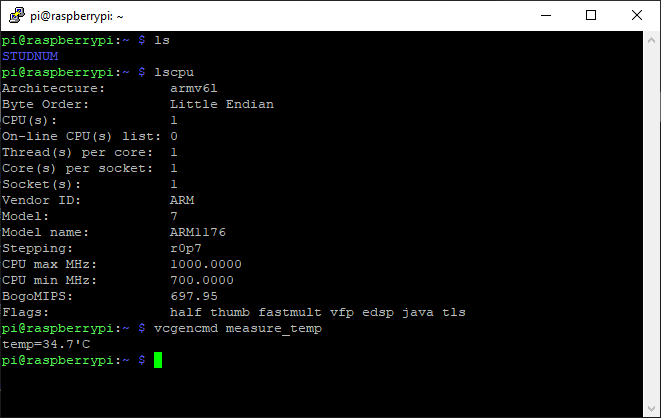
\includegraphics[width=0.8\columnwidth]{Figures/CMDOutput}
\caption{Example output after running the \textbf{ls}, \textbf{lscpu} and \textbf{vcgencmd measure\_temp} command}
\label{fig:CMDOutput}
\end{figure}
%Change pic or just remove it for the ultimate challenge they dont need our help let them suffer

Answer the following questions related to Git:
\begin{enumerate}
    \item What is the purpose of using Git?
    \item List the four commands you would use to commit the file 'changes.txt' (assuming the file has been changed since the last commit) to Git and push it to the GitHub repository https://github.com/fake/link.git
    \item What does it mean for a file to be:
    \begin{enumerate}
        \item untracked
        \item staged
        \item committed
    \end{enumerate}
\end{enumerate}

\subsubsection{Programming Task}
In this task you will develop code to toggle an LED connected to the Pi using a pushbutton.
Be sure to use Git to keep track of changes to your code. For instructions on using Git, refer to the \href{http://wiki.ee.uct.ac.za/Git}{EE Wiki}.
\begin{itemize}
\itemsep0em 
    \item Start by connecting to your Pi.
    \item If not installed, install the Python GPIO libraries, as explained \href{https://pythonhosted.org/RPIO/}{here}. (They should be installed by default.)
    \item Connect 1 LED and 1 pushbutton to the GPIO pins of the Pi - taking care of which pins to use. Look at \href{pinout.xyz}{pinout.xyz} and be sure to not use special purpose pins.
    \item Read about Python Tips and Tricks on the \href{http://wiki.ee.uct.ac.za/RaspberryPi:ProgrammingInPython}{EE Wiki}.
    \item Write your code. It's suggested you work incrementally, committing your code using git each time you accomplish something. 
    \begin{itemize}
        \item Take a look at the RPI.GPIO examples, available \href{https://sourceforge.net/p/raspberry-gpio-python/wiki/Examples/}{here}.
        \item Start by turning the LED on and off in the main() method. Delay between toggling the GPIO by using something like \verb|time.sleep()|.
        \item Now, use a button to toggle the state of the LED. Read over the wiki for help on debouncing.
        \item Don't forget to clean up any resources you might have used at the end of your code!
    \end{itemize}
    \item Push your code to GitHub.
    % \item Submit a PDF with the link to your GitHub repository as per the deliverables section (don't forget to make your repo public).
\end{itemize}

% \subsection{Mark Allocations}
% Marks will be given for:
% \begin{itemize}
% \itemsep0em 
%     \item Correctly completing the terminal task
%     \item Well structured and commented code
%     \item Meaningful git commit messages
%     \item Working code
% \end{itemize}
% Marks will be deducted for:
% \begin{itemize}
% \itemsep0em 
%     \item Not using interrupts and debouncing on your button presses
%     \item Not submitting files in the correct format
%     \item Not linking to the practical on GitHub
%     \item Copying another student's code
%     \item Late submission
% \end{itemize}